\documentclass[dvipdfmx]{report} % 文章の形式を設定
\usepackage[margin=2.5cm]{geometry} % 書式の空白を設定
\usepackage[utf8]{inputenc} % 文字コードをUTF-8に設定
\usepackage{hyperref} % 目次にリンクを付けるため
\usepackage{lipsum} % ダミーテキスト用
\usepackage{tcolorbox} % 枠を利用するため
\usepackage{amsmath} % 数式の記述を行うため
\usepackage{bm} % ベクトルを太字で表示するため
\usepackage{graphicx} % 画像を表示するため
\usepackage{float} % 画像正しい位置で表示するため
\usepackage{tensor} % テンソルを記載するため
\usepackage{multicol} % 複数段落を作成するため
\usepackage{tikz} % 図を作成するため
\usepackage{enumerate} % リストを作成するため
\usepackage{amssymb} % 特殊文字を表示するため
\usepackage{color} % 文字の色を指定するため


\title{降着円盤の像}
\author{大豆生田 幹}
\date{}

\begin{document}

\maketitle % タイトルの作成
\tableofcontents % 目次の作成
\fontsize{11pt}{11pt}\selectfont % 文字サイズの指定

% =================================
% =================================
% =================================
% =================================
% =================================
% 測地線方程式
% =================================
% =================================
% =================================
% =================================
% =================================
\chapter{測地線方程式}

超大質量天体は、降着円盤と呼ばれるガスなどの物質で構成された円盤を持つことが多い。降着円盤は中心天体を高速で公転しており、摩擦の影響で電磁波を放っている。
今回は、重力中心から一定距離に幾何学的に薄い降着円盤を設定し、それがどのように観測されるのかを計算する。

この計算をするためには、光が時空上でどのような軌道を描くのかを知っておかなければならない。これを記述する方程式が、質量のない粒子における測地線方程式であり、まずはこれを導出する。
\section{クラインゴルドン方程式}
$c=0, m=0$において、クラインゴルドン方程式は以下のように書ける
\begin{equation}
\begin{split}
	0 = g^{ij}\nabla_{i}\nabla_{j}\phi(x)
\end{split}
\end{equation}
振動数が非常に大きい波を考えると、波は以下のように書ける
\begin{equation}
\begin{split}
	\phi(x) = C(x)\exp{ \left( \frac{S(x)}{\epsilon}i \right) } \quad \epsilon \ll 1
\end{split}
\end{equation}
これをまとめると、以下のように書ける。
\begin{equation*}
\begin{split}
	0 = g^{jk}(x)\nabla_{j}\nabla_{k}
		\left[ C(x)\exp{ \left( \frac{S(x)}{\epsilon}i \right) } \right]
\end{split}
\end{equation*}

\section{導出}
上記で求めた式を少しづつ計算していく
\begin{equation*}
\begin{split}
	\nabla_k \left[ C(x)\exp{ \left( \frac{S(x)}{\epsilon}i \right) } \right] &= 
		\left[
			( \nabla_k C(x) )
			+ \left( \frac{C(x)}{\epsilon}i \right) (\nabla_k S(x)) 
		\right] \exp \left( \frac{S(x)}{\epsilon} i \right)\\
	\nabla_j \nabla_k \left[ C(x)\exp{ \left( \frac{S(x)}{\epsilon}i \right) } \right] &= 
		[
			\nabla_j \nabla_k C(x)
			+ \frac{2}{\epsilon}i (\nabla_j C(x))(\nabla_k S(x))\\
		& \quad
			+ \frac{C(x)}{\epsilon}i (\nabla_j \nabla_k S(x))
			- \frac{C(x)}{\epsilon ^ 2}i (\nabla_j S(x))(\nabla_k S(x))
		] \exp \left( \frac{S(x)}{\epsilon} i \right)\\
	g^{jk}(x) \nabla_j \nabla_k \left[ C(x)\exp{ \left( \frac{S(x)}{\epsilon}i \right) } \right]
		&=
			g^{jk}(x) \nabla_j \nabla_k C(x) \exp \left( \frac{S(x)}{\epsilon} i \right) \\
		&\quad
			+ \left[
				2(\nabla_j C(x))(\nabla_k S(x)) + C(x) (\nabla_j \nabla_k S(x))
			\right]
			\frac{ g^{jk}(x) }{\epsilon}i \exp \left( \frac{S(x)}{\epsilon} i \right)\\
		&\quad
			- C(x) (\nabla_j S(x))(\nabla_k S(x)) \frac{ g^{jk}(x) }{\epsilon ^ 2}i 				\exp \left( \frac{S(x)}{\epsilon} i \right)
\end{split}
\end{equation*}
ここで書いた項はすべてゼロになるので
\begin{equation*}
\begin{split}
\left\{ \,
\begin{aligned}
	 O(0) &: g^{jk}(x) \nabla_j \nabla_k C(x) = 0\\
	 O(\epsilon^{-1}) &:
	 	2g^{jk}(x)(\nabla_j C(x))(\nabla_k S(x))
		+ g^{jk}(x)C(x) (\nabla_j \nabla_k S(x))\\
   	O(\epsilon^{-2}) &:
		g^{jk}(x) (\nabla_j S(x))(\nabla_k S(x)) = 0\\
\end{aligned}
\right.
\end{split}
\end{equation*}
上の関係式の中で、$O(\epsilon^{-2})$部分は測地線方程式そのものになっている。$O(\epsilon^{-2})$式全体の共変微分をとると
\begin{equation*}
\begin{split}
	0 &= \nabla_j(\nabla^i S(x))(\nabla_i S(x)) \\
	&= 	(\nabla_j \nabla^i S(x))(\nabla_i S(x))
		+ (\nabla^i S(x))(\nabla_j \nabla_i S(x))
\end{split}
\end{equation*}
波数ベクトル$\bold{k}$、アフィンパラメータ$\lambda$に対して以下の関係式が成り立つと仮定する。
\[ \nabla^i S = k^i = \frac{d x^i}{d\lambda} \]
すると、$O(\epsilon^{-2})$式は以下のように書き換えられる。
\[
	0 = (\nabla_j k^i)k_i + k^i(\nabla_j k_i)
\]
\begin{tcolorbox}[title=一般のテンソルに対する共変微分]
\begin{equation*}
\begin{split}
	\nabla_c \tensor{T}{^{a_1 \cdots a_i}_{b_1 \cdots b_j}}  
	&=
		\tensor{T}{^{a_1 \cdots a_i}_{b_1 \cdots b_j, c}}\\
	&\quad
		+ \sum^{m}_{d=1}
		\tensor{\Gamma}{^{a_d}_{fc}}
		\tensor{T}{^{a_1 \cdots a_{d-1} f a_{d+1} \cdots a_i}_{b_1 \cdots b_j}}\\
	&\quad
		- \sum^{m}_{e=1}
		\tensor{\Gamma}{^{f}_{b_e c}}
		\tensor{T}{^{a_1 \cdots a_i}_{b_1 \cdots b_{e-1} f b_{e+1} \cdots b_j}}\\
\end{split}
\end{equation*}
\end{tcolorbox}
共変微分が上記のように書けたことを思い出すと、式は以下のようにまとめられる。これが質量のない物質における測地線方程式である。
\[
0 = \frac{d^2 x^a}{d \lambda^2} + \tensor{\Gamma}{^{a}_{bc}}\frac{dx^b}{d\lambda}\frac{dx^c}{d\lambda}
\]

% =================================
% =================================
% =================================
% =================================
% =================================
% シュワルツシルト解
% =================================
% =================================
% =================================
% =================================
% =================================
\chapter{シュワルツシルト解}
一般相対論による強い重力の効果は、シュワルツシルト時空と呼ばれる球対称真空のブラックホール解を典型的な例として理解できる。シュワルツシルト時空の線素は以下のように書くことができる。

\[
ds^2 =
		-\left( 1 - \frac{2M}{r} \right)dt^2
		+ \left( 1 - \frac{2M}{r} \right)^{-1}dr^2
		+ r^2( d\theta^2 + \sin^2\theta d\phi^2 )
\]
この解は$r \rightarrow \infty$で漸近的にミンコフスキー時空に近づく。

% =================================
% 真空におけるアインシュタイン方程式の確認
% =================================
\section{解の確認}
参考に書く:https://eman-physics.net/relativity/schwarzschild.html 

% =================================
% 光の軌道が満たす微分方程式の導出
% =================================
\section{光の軌道が満たす微分方程式の導出}

% =================================
% =================================
% =================================
% =================================
% =================================
% ブハダール解
% =================================
% =================================
% =================================
% =================================
% =================================
\chapter{ブハダール解}

% =================================
% ブハダール解
% =================================
\section{ブハダール解}



/////////////////////////////////////////////////////////////////////////\\
/////////////////////////////////////////////////////////////////////////
\textcolor{red}{テスト}

% 方程式
\begin{equation*}
\begin{split}
	\bar{w}_j = \left( \right) \int^{}_{}
\end{split}
\end{equation*}

% ボックス
\begin{tcolorbox}[title=メモ用]
\begin{eqnarray*}
	1 = 0
\end{eqnarray*}
\end{tcolorbox}

% { 付き方程式
\begin{equation}
\left\{ \,
\begin{aligned}
	1 &= 0\\
	1 &= 0\\
\end{aligned}
\right.
\end{equation}

% 行列
\[
\left(
\begin{matrix}
a & b \\
c & d
\end{matrix}
\right)
\]


% 画像
\begin{figure}[H]
    \centering
    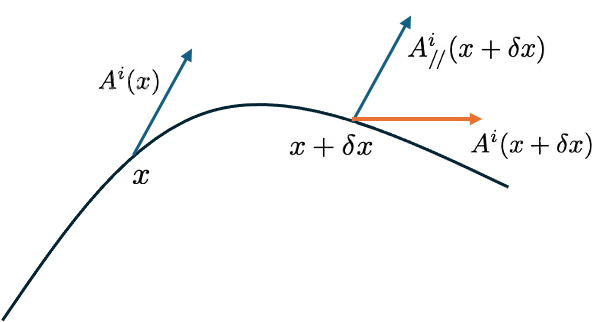
\includegraphics[width=0.5\columnwidth]{./images/0106/01.png}
    \caption{並行移動}
    \label{}
\end{figure}

% リスト
\begin{enumerate}[(1)\,]
\item{}
\end{enumerate}

\end{document}